\section{Tafeldetektierung}

Das folgende Kapitel befasst sich mit dem ersten Schritt in der automatisierten Analyse der Grabungsfotos: der Erkennung der Schiefertafeln.\\
Zunächst sollen die Tafeln vorgestellt und die Probleme bei der Detektion erörtert werden. Im Anschluss werden verschiedene Möglichkeiten der Erkennung präsentiert. Schließlich werden mehrere angewandte Methoden erörtert und die erzielten Ergebnisse vorgestellt.

\subsection{Die Tafeln und ihre Tücken}

\subsubsection{Die Tafeln}

Die Verwendung von Tafeln zur Dokumentation von Fund- und Grabungsarealen ist in allen, im weitesten Sinne grabenden, Wissenschaften weit verbreitet (Vgl. Bildquellen) . So setzt auch die Archäologie diese Methode ein. Dabei werden neben den zu dokumentierenden Gebieten verschiedenste Formen von Tafeln oder Schildern platziert, auf denen Zeit und Ort der Aufnahme sowie weitere bild- und motivbezogene Informationen festgehalten werden können. Der Vielfalt von Form und Material der Tafeln ist dabei keine Grenze gesetzt.
Bei den Tafeln, die Gegenstand dieses Projektes sind, handelt es sich um Schiefertafeln mit einem Holzrahmen, die mit Kreide beschriftet wurden. Für die Detektion der Tafeln ergeben sich daraus folgende Faktoren:\\
\begin{enumerate}
\item Die Tafeln haben grundsätzlich eine rechteckige Form.
\item Durch die breite des Rahmens können bis zu zwei Rechtecke erkannt werden, ein Inneres und ein Äußeres.
\item Durch die große Differenz zwischen dem hellen Holzrahmen und der dunklen Schieferplatte sollte der innere Rand in der Regel gut detektierbar sein.
\end{enumerate}
\begin{SCfigure}[0.5][h!]
\caption{Beispiel eines Fotos der verwendeten Tafel. GOT bezeichnet die Kampagne, darunter folgt das Datum. US ist die Abkürzung für \textit{unità stratigrafica}, die stratigrafische Einheit.}
\includegraphics[width=0.6\textwidth]{catacom_1020_cutout.png}
\end{SCfigure}

Die im Beispielbild gezeigte Tafel stellt gewissermaßen ein Idealbild dar: Die Tafel nimmt einen relativ großen Teil des Originalbildes -- bei der Darstellung hier handelt es sich um einen Ausschnitt -- ein. Sie ist frontal vor der Kamera positioniert. Die Beleuchtung ist gut und indirekt. Keines der weiteren Bildelemente verdeckt die Tafel.
Diese Beschreibung impliziert schon die Problemfelder, die bei der Detektion beachtet werden müssen:
\begin{enumerate}
\item Die Tafel ist unter Umständen stark rotiert.
\item Die Distanz der Tafel zur Kamera und damit ihre Größe im Bild kann stark variieren.
\item Der Rahmen der Tafel kann teilweise verdeckt oder anderweitig durch Gegenstände überlagert sein.
\item Die Farbe des Tafelrahmens kann dazu führen, dass sie sich nicht klar vom Hintergrund abhebt, was die Detektion des äußeren Randes erschweren kann.
\item Unregelmäßigkeiten im Rahmen, die auf grobe Verarbeitung oder Abnutzung zurückzuführen sind, können die Detektion erschweren.
\item Die Beleuchtung kann zu Problemen führen. Grundsätzlich sind alle Fotos hell und gut ausgeleuchtet, direktes Licht kann sich aber negativ auf die Kontraste auswirken.
\item Weitere Gegenstände, die den Spezifika der Tafeln entsprechen, können im Bild vorhanden sein.
\end{enumerate}

Teilweise werden die hier genannten Probleme auch bei der Texterkennung wieder relevant. Auf diese und auf weitere wird an geeigneter Stelle zurückgegriffen.

\subsubsection{Tafelvergleiche}

Im Rahmen der Arbeit wurden weitere Tafeln exemplarisch dem Algorithmus unterzogen. Dabei handelte es sich um Aufnahmen der späteren Grabungen des Deutschen Archäologischen Institutes am Kapitol in Rom sowie um vergleichbare Fotos von Bodenuntersuchungen der Gruppe Terrestrische Ökohydrologie der Friedrich-Schiller-Universität Jena. Der ursprüngliche Gedanke dahinter war eine möglichst universale Detektion von Tafeln aller Art anzustreben. Während dieses Vorhaben aus Zeit- und Komplexitätsgründen ohnehin zum Scheitern verurteilt war, warf das weitere Material die Frage auf, wo die Grenze des technisch möglichen liegt, vor allem mit der hier letztlich gewählten Methodik.\\

Die Tafeln beider Projekte sollen im Folgenden kurz vorgestellt werden, um das Spektrum der Komplexität 
evtl. Vergleiche zu Tafeln aus späterer Grabung als Positivbeispiel:\\
besser gearbeitete Tafeln\\
besser lesbare Schrift\\
evtl. Vergleiche zu Tafeln der Bodenkunde als Negativbeispiel:\\
Tafel schwierig durch Form und Farbe\\
Klarsichthülle: Reflektion und Formveränderung\\
oft verdeckt\\

\subsection{Detektierungsmöglichkeiten}

\subsubsection{CNN}

CNN\\

Convolutional Neural Networks (CNN) Kurzdefinition\\

Coco und Coco bzw. Yolo Weights erklären\\

Code Herkunft erklären (Rücksprache Sellent bzgl. Quelle und Zitation etc.)\\

\subsubsection{Ergebnisse CNN}

Der Ansatz bei der Arbeit mit CNNs bestand in der Überlegung, dass die Tafeln bestimmten Objekten, wie beispielsweise Bücher oder Müslipackungen, ausreichend ähneln, um als solche erkannt zu werden. Prinzipiell wäre es auch möglich, ein eigenes Modell zu trainieren, dass auf die Erkennung der Tafeln zugeschnitten ist. Dieser Ansatz wurde hier nicht weiter verfolgt, da einerseits die vorliegende Datenmenge von knapp 1500 Bildern gering für ein solches Vorhaben ist und andererseits der Aufwand sehr groß wäre für ein Problem, das sich mit klassischen Methoden der Computer Vision ohne Weiteres lösen lässt.\\

Entsprechend wurden sowohl der YOLO, als auch der COCO object detector auf den Datensatz angewandt. Die Ergebnisse sind dabei wenig überzeugend.

\begin{SCfigure}[0.75][h!]
\caption{Eine beispielhafte Auswertung mit COCO-Weights: Es werden zwar durchaus Objekte erkannt, die Tafel ist aber nicht darunter. Die Objekte werden nicht korrekt erkannt, was aber bei dieser untypischen Fotografie nicht weiter verwunderlich ist.}
\includegraphics[width=0.5\textwidth]{coco_fail.PNG}
\end{SCfigure}

\begin{SCfigure}[0.75][h!]
\caption{Auffällig häufig ist die Klassifizierung des Nordungspfeils als Surfbrett. Diese ist aber nicht häufig und zuverlässig genug, um COCO zur Erkennung des Pfeils einzusetzen.}
\includegraphics[width=0.5\textwidth]{coco_surfboard.PNG}
\end{SCfigure}

\begin{SCfigure}[0.75][h!]
\caption{Ähnlich wie bei COCO klassifiziert auch YOLO die Tafeln nur auf wenigen Bilder. Dann allerdings als Scheren...}
\includegraphics[width=0.5\textwidth]{scissors.PNG}
\end{SCfigure}

\begin{SCfigure}[0.75][h!]
\caption{... oder als Sportgerät. Die erhoffte Ähnlichkeit mit beschrifteten, rechteckigen Objekten wie Büchern besteht somit also nicht.}
\includegraphics[width=0.5\textwidth]{sportsball.PNG}
\end{SCfigure}

\subsubsection{Ergebnisse Feature Detection}

theoretische Grundlagen Feature Detection\\

\subsubsection{Ergebnisse Feature Detection}

alten Code raussuchen, aufbereiten und präsentieren\\

\subsubsection{Contours}

Die Contours-Funktion von OpenCV basiert darauf, dass alle benachbarten Punkte mit gleicher Farbe oder Intensität als Teil einer Kontur betrachtet werden (Quelle OpenCV doc). Der Algorithmus liefert also eine Liste von Punkten, die Grundlage einer Vektorgrafik sind. Der Parameter
\begin{verbatim}
cv2.CHAIN_APPROX_SIMPLE
\end{verbatim}
vereinfacht die Kontur, indem redundante Punkte entfernt werden. Als Input für Contours werden binarisierte Bilder empfohlen. Das sind Bilder, die in eine Grauskala umgewandelt  und anhand eines Thresholds, eines Grenzwertes, in ein reines Schwarz-Weiß-Bild transformiert wurden. Zur Binarisierung wurden im Verlauf der Entwicklung zwei Verfahren geschrieben, von denen eines de facto nicht mehr in Verwendung ist, der Vollständigkeit halber hier aber aufgeführt werden soll.
Das Kernproblem, das zu der parallelen Entstehung zweier Konzepte führte, waren vor allem falsch-positive Detektionen von Tafeln, also Fälle, in denen korrekterweise Rechtecke erkannt wurden, die aber keine Tafeln waren.
\begin{SCfigure}[0.5][h!]
\caption{Falsch-Positive: Hier werden korrekterweise Rechtecke detektiert, die allerdings keine Tafeln und somit uninteressant für die weitere Verarbeitung sind.}
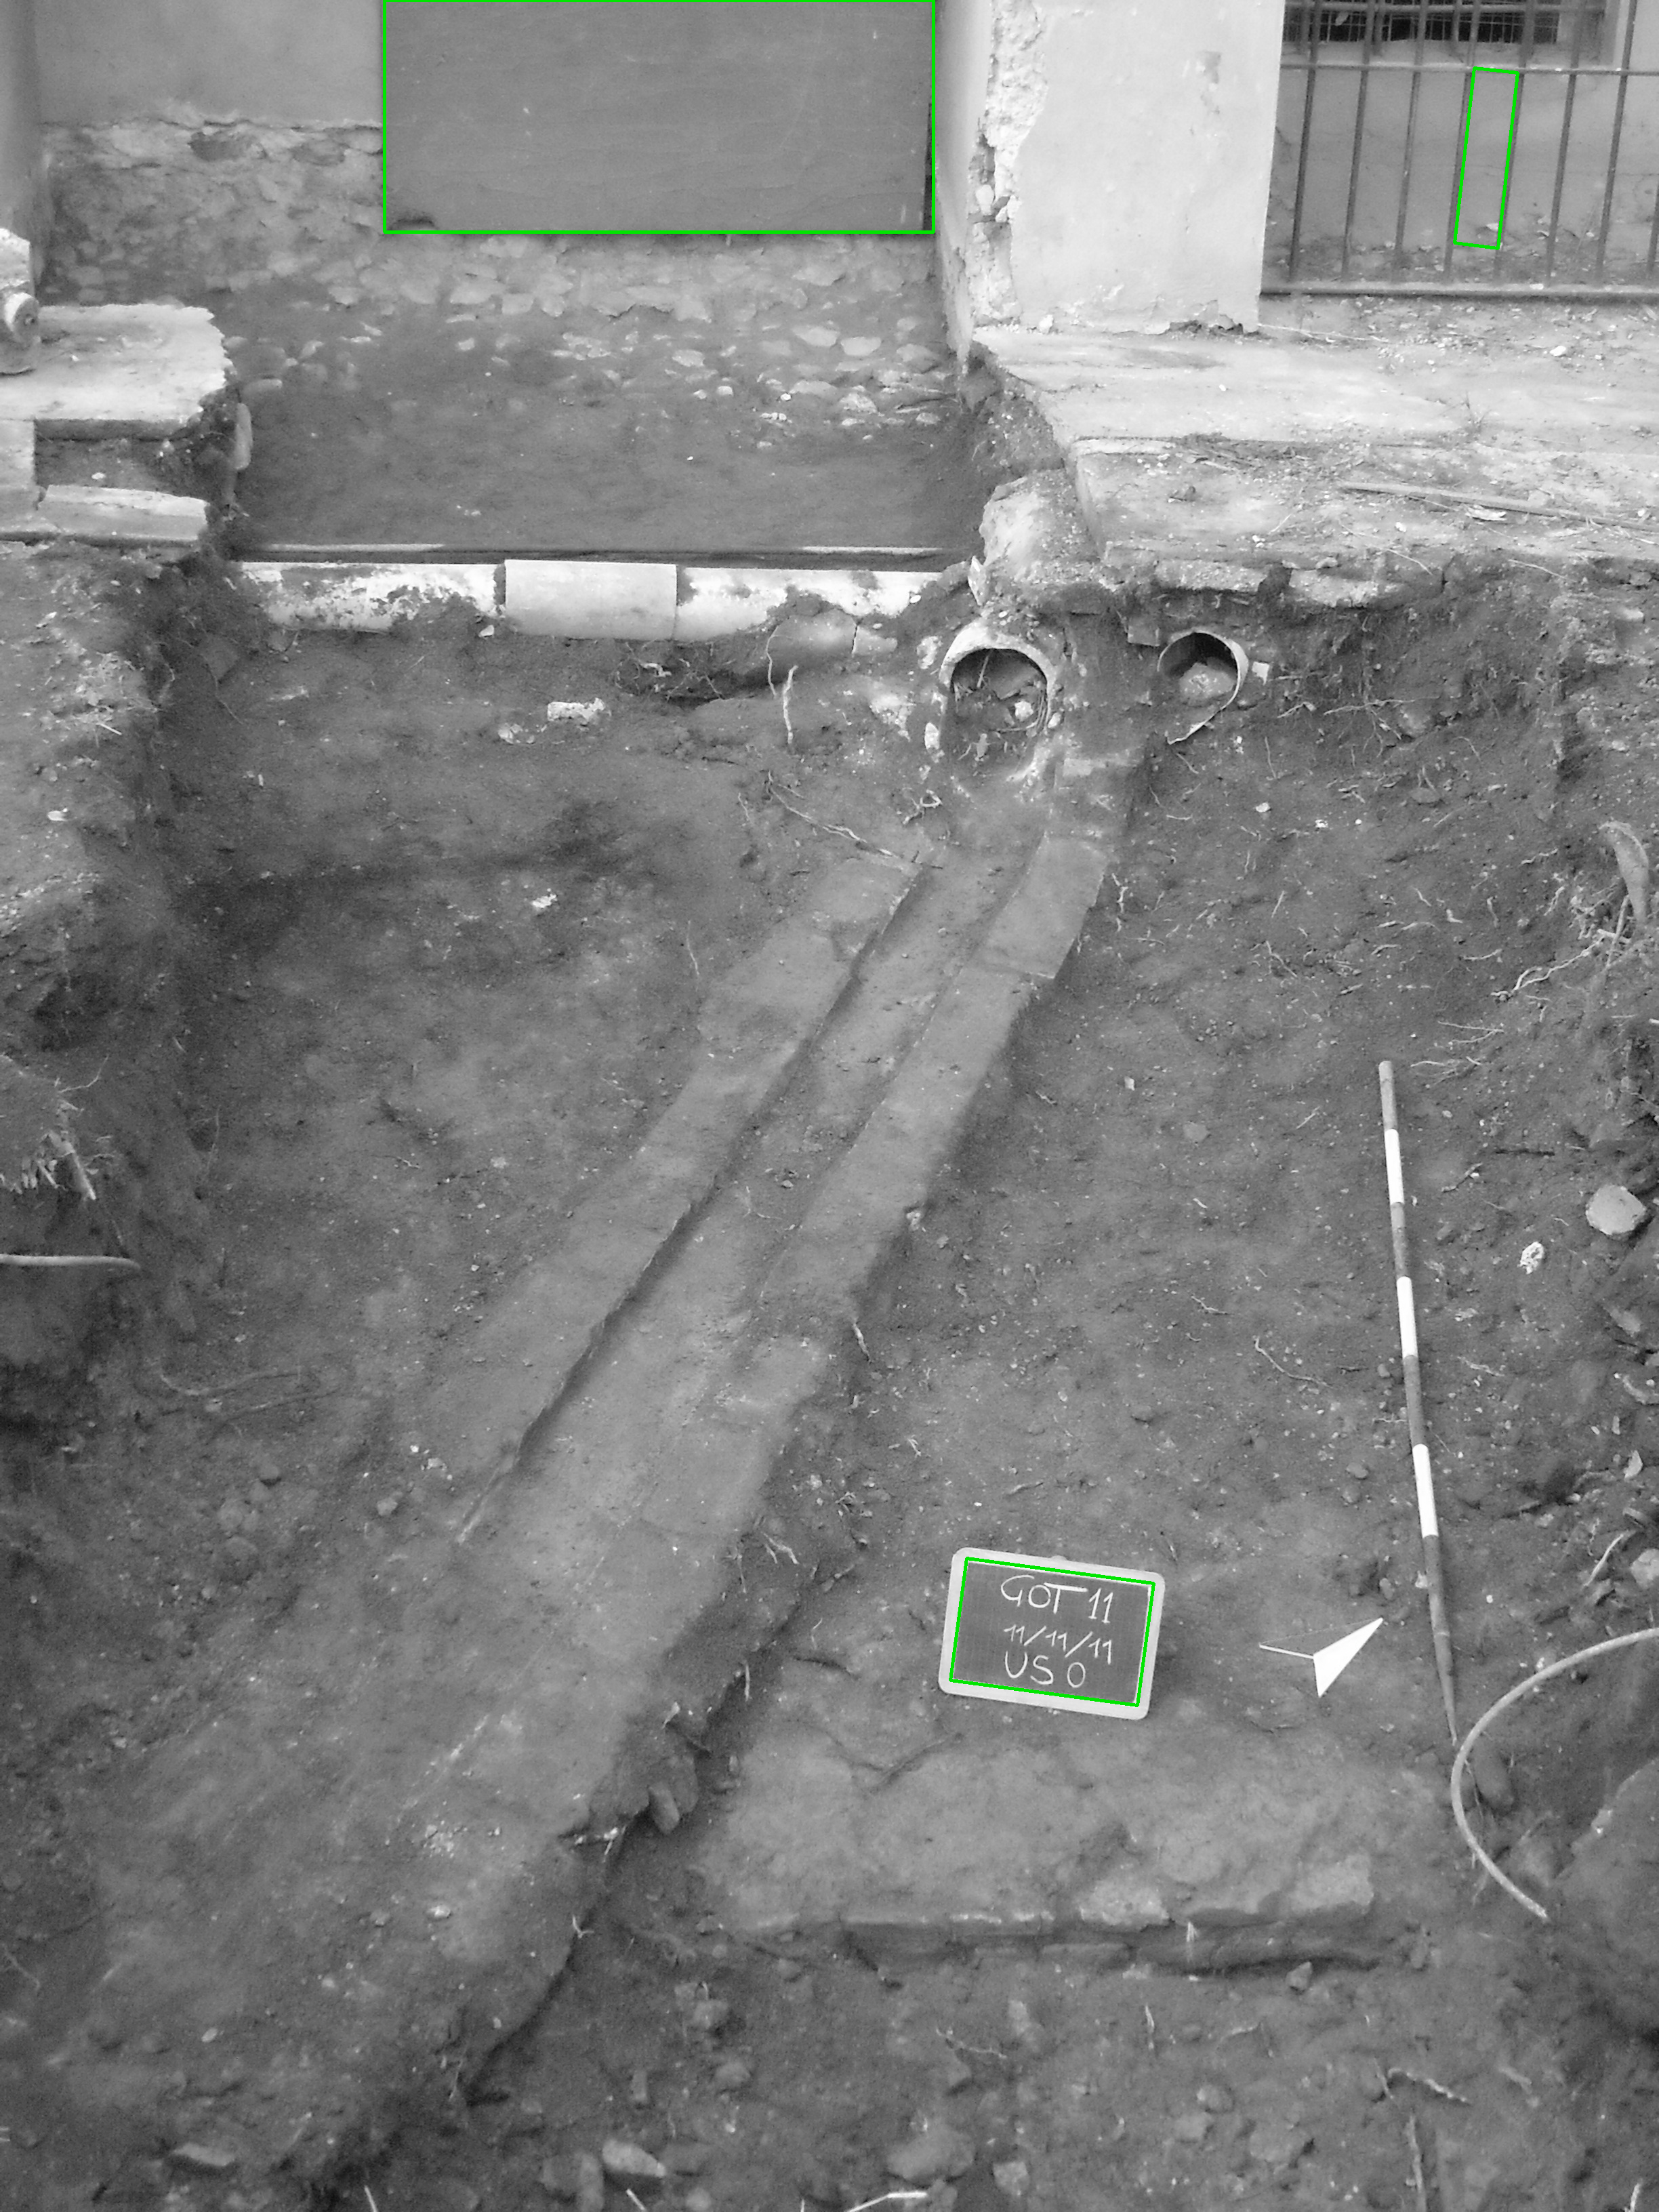
\includegraphics[width=0.5\textwidth]{catacom_1023_adaptive.png}
\end{SCfigure}

\subsubsection*{ Adaptive Ansatz}
Der adaptive Ansatz heißt so aufgrund der Verwendung eines adaptiven Thresholds, der auf Bildausschnitten vorher festgelegter Größe gewissermaßen lokale Thresholds festlegt und so gut geeignet ist, um Bilder mit großen Unterschieden in der Helligkeit zu binarisieren, ohne dass wichtige Informationen verloren gehen (Quelle OpenCV doc). Da es bei dem vorliegenden Material, vor allem aufgrund von Schatten und direktem Sonnenlicht, große Helligkeitsunterschiede sowohl zwischen den Bildern als auch innerhalb eines einzelnen Bildes gibt, ist die Arbeit mit einem fixen Threshold schwierig und dieser Ansatz bot sich an. Allerdings entstand dadurch eine relativ große Zahl an falsch-positiven, wie oben zu sehen. So kam es zur Entwicklung des zweitens Ansatzes.\\

\subsubsection*{ Iterative Ansatz}
Der Iterative Ansatz ist danach benannt, dass durch ein Spektrum an Thresholds iteriert wird. In jedem dieser so entstandenen binären Bilder werden anschließend die Contours gesucht und aus diesen wiederum die Rechtecke ausgewählt. Die Idee dahinter war, dass die Falsch-Positiven oft weniger konstant in den Bildern detektiert wurden als die tatsächlichen Tafeln. Würde man also ein Bild mit verschiedenen Thresholds binarisieren sollte das Rechteck, dass in den meisten dieser binären Bilder entdeckt wird, die Tafel sein. In der Implementierung dieses Ansatzes werden von 20 bis 200 in Fünferschritten 37 Thresholds durchlaufen. Die Gleichheit zweier Rechtecke wird dabei mittels \textit{Intersection over Union} berechnet, deren Ergebnis sich der 1 nähert, je gleicher die Rechtecke in Position und Größe sind.
Tatsächlich können mit diesem Verfahren die Zahl der Falsch-Positiven reduziert werden, ohne das Problem allerdings ganz zu lösen. Generell lässt sich sagen, dass je öfter ein Rechteck in einer der Iterationen erkannt wird, desto größer ist die Wahrscheinlichkeit, dass es sich tatsächlich um eine Tafel handelt. Ab einem Wert von 20 liegt die Quote bei 100\%. Es gibt aber auch korrekt erkannte Tafeln, die nur in 6 der Iterationen detektiert werden und umgekehrt Falsch-Positive, die in bis zu 14 Iterationen vorkommen. Zwar handelt es sich hier jeweils um Ausreißer, das Problem bleibt jedoch bestehen. Empirisch hat sich gezeigt, dass alles unter 6 Iterationen mit Sicherheit keine Tafel ist und somit aussortiert werden kann. Wenige Ausreißer verhindern, dass diese Grenze nach oben gesetzt werden kann. Auch dieser Ansatz führte also nicht zum gewünschten Ergebnis.
\begin{SCfigure}[0.5][h!]
\caption{Falsch-Positive beim Iterativen Ansatz. Hier wurden in 14 Iterationen die Holzbretter als Rechteck identifiziert.}
\includegraphics[width=0.5\textwidth]{catacom_1083_14.png}
\end{SCfigure} \begin{SCfigure}[0.5][h!]
\caption{Direkte Sonneneinstrahlung macht die Erkennung schwierig, vor allem, da sich der Rahmen nicht mehr stark vom Schiefer abhebt. Nur in 6 Iterationen wurde diese Tafel erkannt.}
\includegraphics[width=0.5\textwidth]{catacom_1162_6.png}
\end{SCfigure}\\
\subsubsection{Hough}

Später schreiben, je nachdem ob sich der Algorithmus verbessern lässt und präzisere Ergebnisse zu erzielen als simple crop oder nicht. In letzterem Falle Ansatz und Fehlschlag vorstellen.\\

\subsubsection{Ergebnisse Kantenerkennung /Contours}
Detaillierte Beschreibung des Vorgehens\\
Vor- und Nachteile aufzählen\\
konkrete Probleme bennen\\
